\section{Data collection and characterization}
\label{sec:6_2_data}

Here I characterize system usage in all the case of study cities, focusing on those metrics that are instrumental for the design of FFCS systems based on electric vehicles and highlighting the non-stationary patterns. 

%\subsection{Data collection and filtering}
%\label{par:coll_and_filter}
%The modern FFCS provider like Car2go, DriveNow or GoGet use information systems to expose the position of the available cars through web services. Customers access these to check  which cars are available for a rental by using a smartphone app. For instance, Car2go offers public Application Programming Interface (API) \footnote{car2goAPI, \url{https://www.car2go.com/api/tou.htm} service subject to approval by car2Go. Approval granted in Sept. 2016 and discontinued in Jan. 2018.} to access the information about the system status. We use these APIs to collect data about actual rentals occurred over time following a streaming approach. First, we get the operative area for each city, i.e., the zone where cars can be rented and returned. The operative areas remain constant for several months.
%Next, we collect a snapshot every minute reporting the positions of all cars available for a rental, for each city. From each snapshot we save the car plates (used as car identifier) and its geographic coordinates.
%
%We developed UMAP~\cite{UMAP}, a software able to process these snapshots and rebuild, for each car, the history in terms of \emph{bookings} and \emph{parkings}.\footnote{UMAP can be downloaded from \url{https://github.com/MobilityPolito/UMAP}}
%A booking is an event describing a possible car rental $i$, characterized by the starting and final position $o(i)$ and $d(i)$, and starting and ending time $t_s(i)$ and $t_e(i)$. A parking describes a period of time when the car was parked and available for rentals; it is characterized by the location and the starting and final time. In a nutshell, we process the snapshots of the available cars and derive booking periods by observing which cars are available at each snapshot.
%Given a car, when it ``disappears'' from a snapshot, it means that someone has booked it -- so that the car is not available for other customers. A new booking is started. When the same car ``reappears'' back later on, it means someone has returned it. The booking is then ended.
%
%Not all bookings correspond to actual rentals:
%(i) a customer can book a car, and cancel the booking later on;
%(ii) the data collection may suffer from outages, so that some snapshots may miss some available cars;
%(iii) cars may go in maintenance, so that they disappear and never come back (or return after a long time).
%We developed data cleaning and filtering rules to extract actual \textit{rentals} from bookings. A booking is considered a valid rental if:
%(i) it lasts at least 3 minutes;
%(ii) the ending position is at least 700\,m far from the staring position, with both positions inside the city operative area;\footnote{This to account for possible errors in the GPS fixing, and to remove rentals started and ended in different cities.};
%(iii) its duration is smaller than 1\,h. These thresholds have been selected by domain knowledge of the data -- see~\cite{UMAP} for more details.
%Bookings that do not correspond to rentals are then merged with parkings events (since the car did not move).
%
%We started to collected data in December 2016 in all the 22 cities in which Car2go is present, and stopped our collection in February 2018. Overall, we obtained more than 28 millions rentals and parkings that we leverage for our studies.

\subsection{Temporal characterization}
I collected the data with the software described in chapter \ref{chap:2_dataset}. Reminding that not all bookings correspond to an actual rental because:
\begin{itemize}
	\item a customer can book a car, and cancel the booking later on;
	\item the data collection may suffer from outages, so that some snapshots may miss some available cars;
	\item cars may go in maintenance, so that they disappear and never come back (or return after a long time)
\end{itemize}
%(i) a customer can book a car, and cancel the booking later on;
%(ii) the data collection may suffer from outages, so that some snapshots may miss some available cars;
%(iii) cars may go in maintenance, so that they disappear and never come back (or return after a long time).
I developed data cleaning and filtering rules to extract actual \textit{rentals} from bookings. A booking is considered a valid rental if:
\begin{itemize}
	\item it lasts at least 3 minutes;
	\item the ending position is at least 700\,m far from the staring position, with both positions inside the city operative area;\footnote{This to account for possible errors in the GPS fixing, and to remove rentals started and ended in different cities.};
	\item its duration is smaller than 1\,h. These thresholds have been selected by domain knowledge of the data -- see~\cite{ciociolaumap} for more details.
	\item \mc{rivedere capitolo appropriato con vari link, e linkare anche le def}
\end{itemize}
Bookings that do not correspond to rentals are then merged with parkings events (since the car did not move).

%I started to collected data in December 2016 in all the 22 cities in which Car2go is present, and stopped our collection in February 2018. Overall, we obtained more than 28 millions rentals and parkings that we leverage for our studies.

In this work I focus the analysis from September to November 2017 in four city: Turin (Italy), Milan (Italy), Berlin (Germany), Vancouver (Canada).
Overall, the case study dataset has more than 1 million rental events that describe the typical usage patterns of FFCS customers. 


\begin{figure}[t]
    \begin{center}
        \begin{subfigure}{\textwidth}
            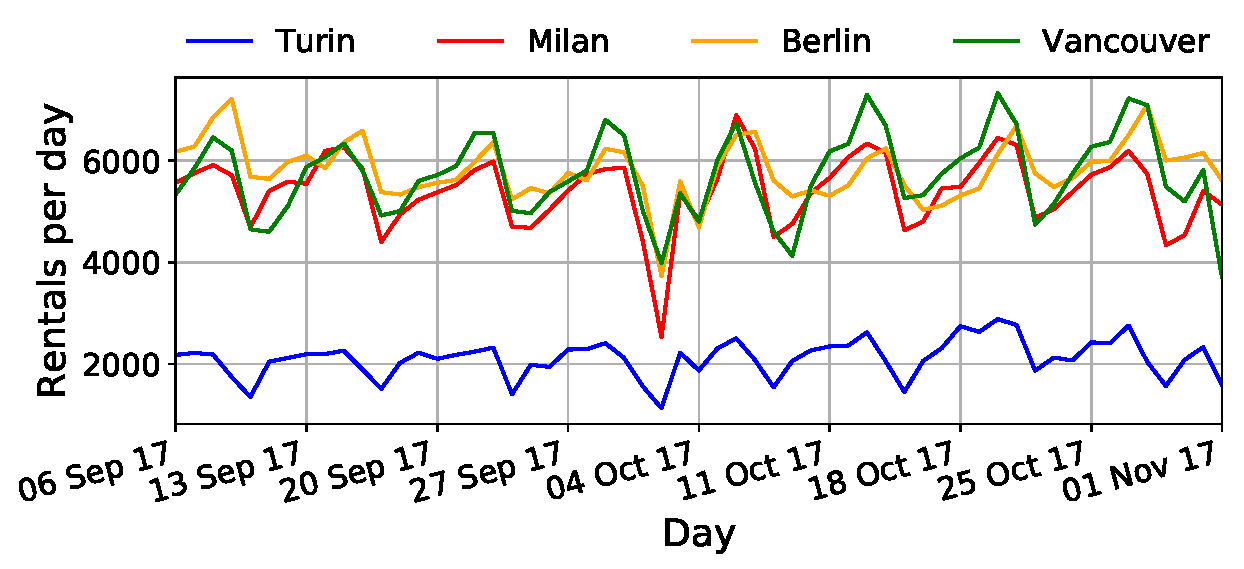
\includegraphics[width=\columnwidth]{figures/bookings_per_day.pdf}
            \caption{Number of rentals per day.}
            \label{fig:rentals_per_day}
        \end{subfigure}
         \begin{subfigure}{\textwidth}
             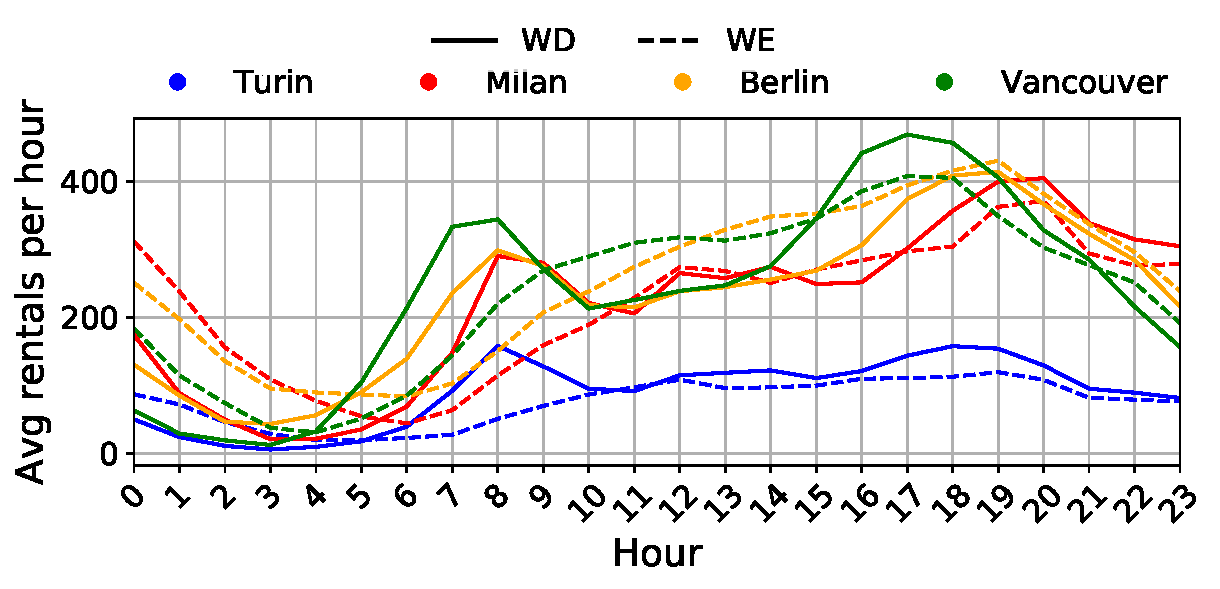
\includegraphics[width=\columnwidth]{figures/aggBookginfsPerHour.pdf}
             \caption{Average number of rentals per hour.}
             \label{fig:rentals_per_hour}
         \end{subfigure}
         \caption{Rental trends in different cities.}
         \label{fig:rentals_trends}
\end{center}
\end{figure}


\begin{figure}[t]
%     \begin{center}
            \begin{subfigure}{\textwidth}
            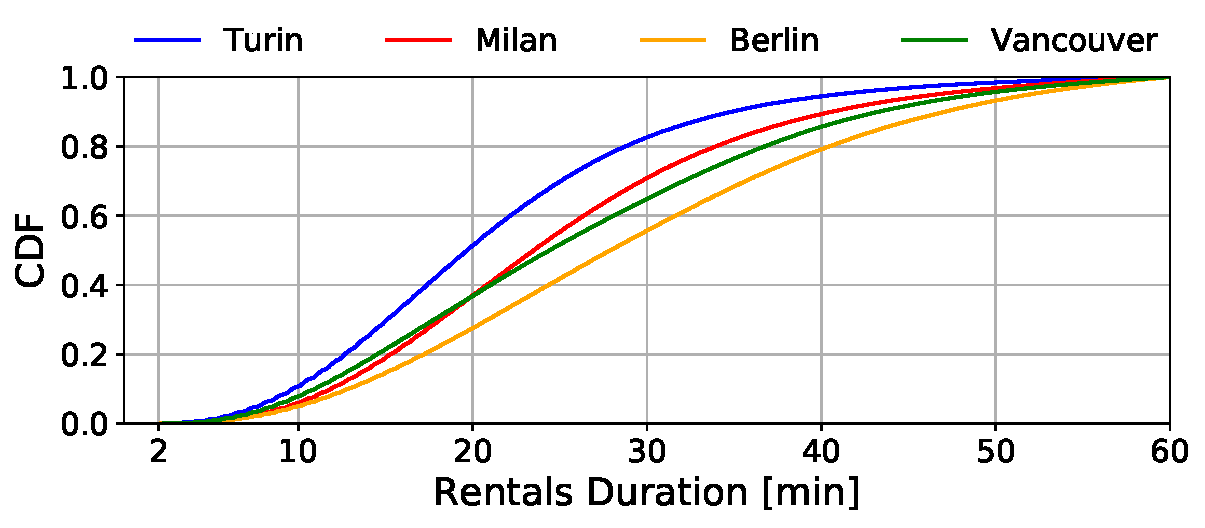
\includegraphics[width=\columnwidth]{figures/CDF_aggregate_RentalsDuration.pdf}
           % \caption{CDF of driving duration}
            %\label{fig:cdf_driving_duration}
\vspace{-0.3cm}
        \end{subfigure}\\
        \begin{subfigure}{\textwidth}
             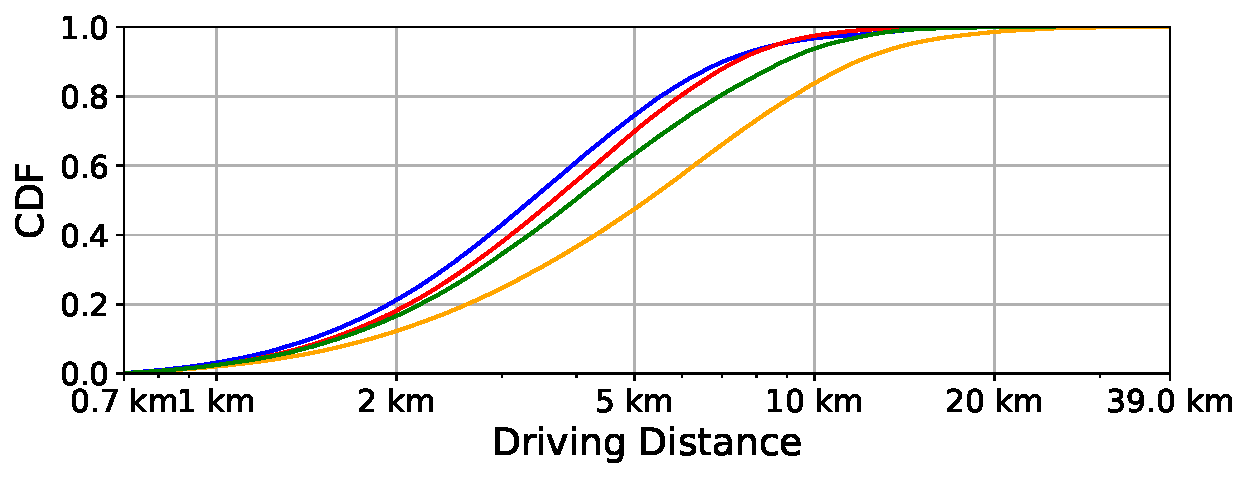
\includegraphics[width=\columnwidth]{figures/CDF_aggregate_RentalsDistance.pdf}
           %  \caption{CDF of driving distance}
            % \label{fig:cdf_driving_distance}
\vspace{-0.3cm}
         \end{subfigure}\\
         \begin{subfigure}{\textwidth}
             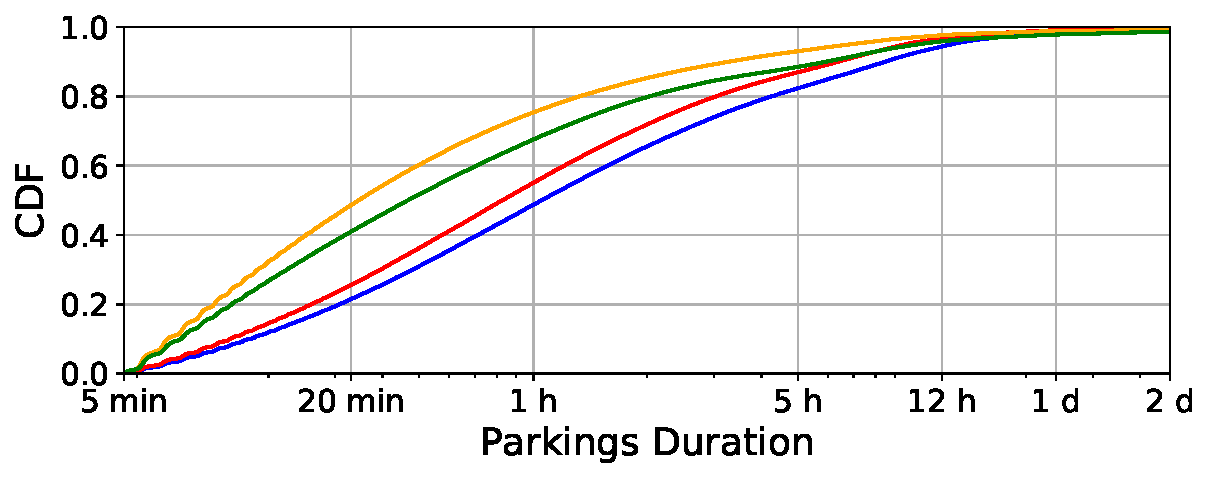
\includegraphics[width=\columnwidth]{figures/CDF_aggregate_ParkingsDuration.pdf}
           %  \caption{CDF of parking duration}
            % \label{fig:cdf_parking_duration}
         \end{subfigure}
         
         \caption{Car Sharing usage habit characterization.}
         \label{fig:cdf_characterization}
% \end{center}
\end{figure}

To give the intuition of the system, I first provide a characterization of actual usage patterns by current FFCS customers in each city. I focus first on the temporal characteristics.
Figure~\ref{fig:rentals_trends} reports the rental trend. More in details, figure~\ref{fig:rentals_per_day} shows the number of recorded rentals for each day in the considered period. Usage similarity is striking, with Milan, Berlin and Vancouver that have more rentals per day than Turin. This intense usage, justify the difference in fleet size between the cities, with these three having at least twice as much cars with respect to Turin (see Tab.~\ref{tab:summary}). These first results highlights the importance of extending the users' pattern analyses of same provider on different cities. A second interesting aspect is the presence of a weekly pattern: in correspondence of the weekends the number of rentals drops of about 30\%. This is justified by the fact that during the working days cars are used for commuting. Moreover, non-stationary events due to holidays or strikes are visible, e.g., October 6th in Milan due to a public transport strike.\footnote{The sudden fall around the October $2^{th}$ is due to system outage that caused a lack of data.} 

\begin{figure*}[t!]
    \begin{center}
        \begin{subfigure}{\textwidth}
		    \begin{center}
            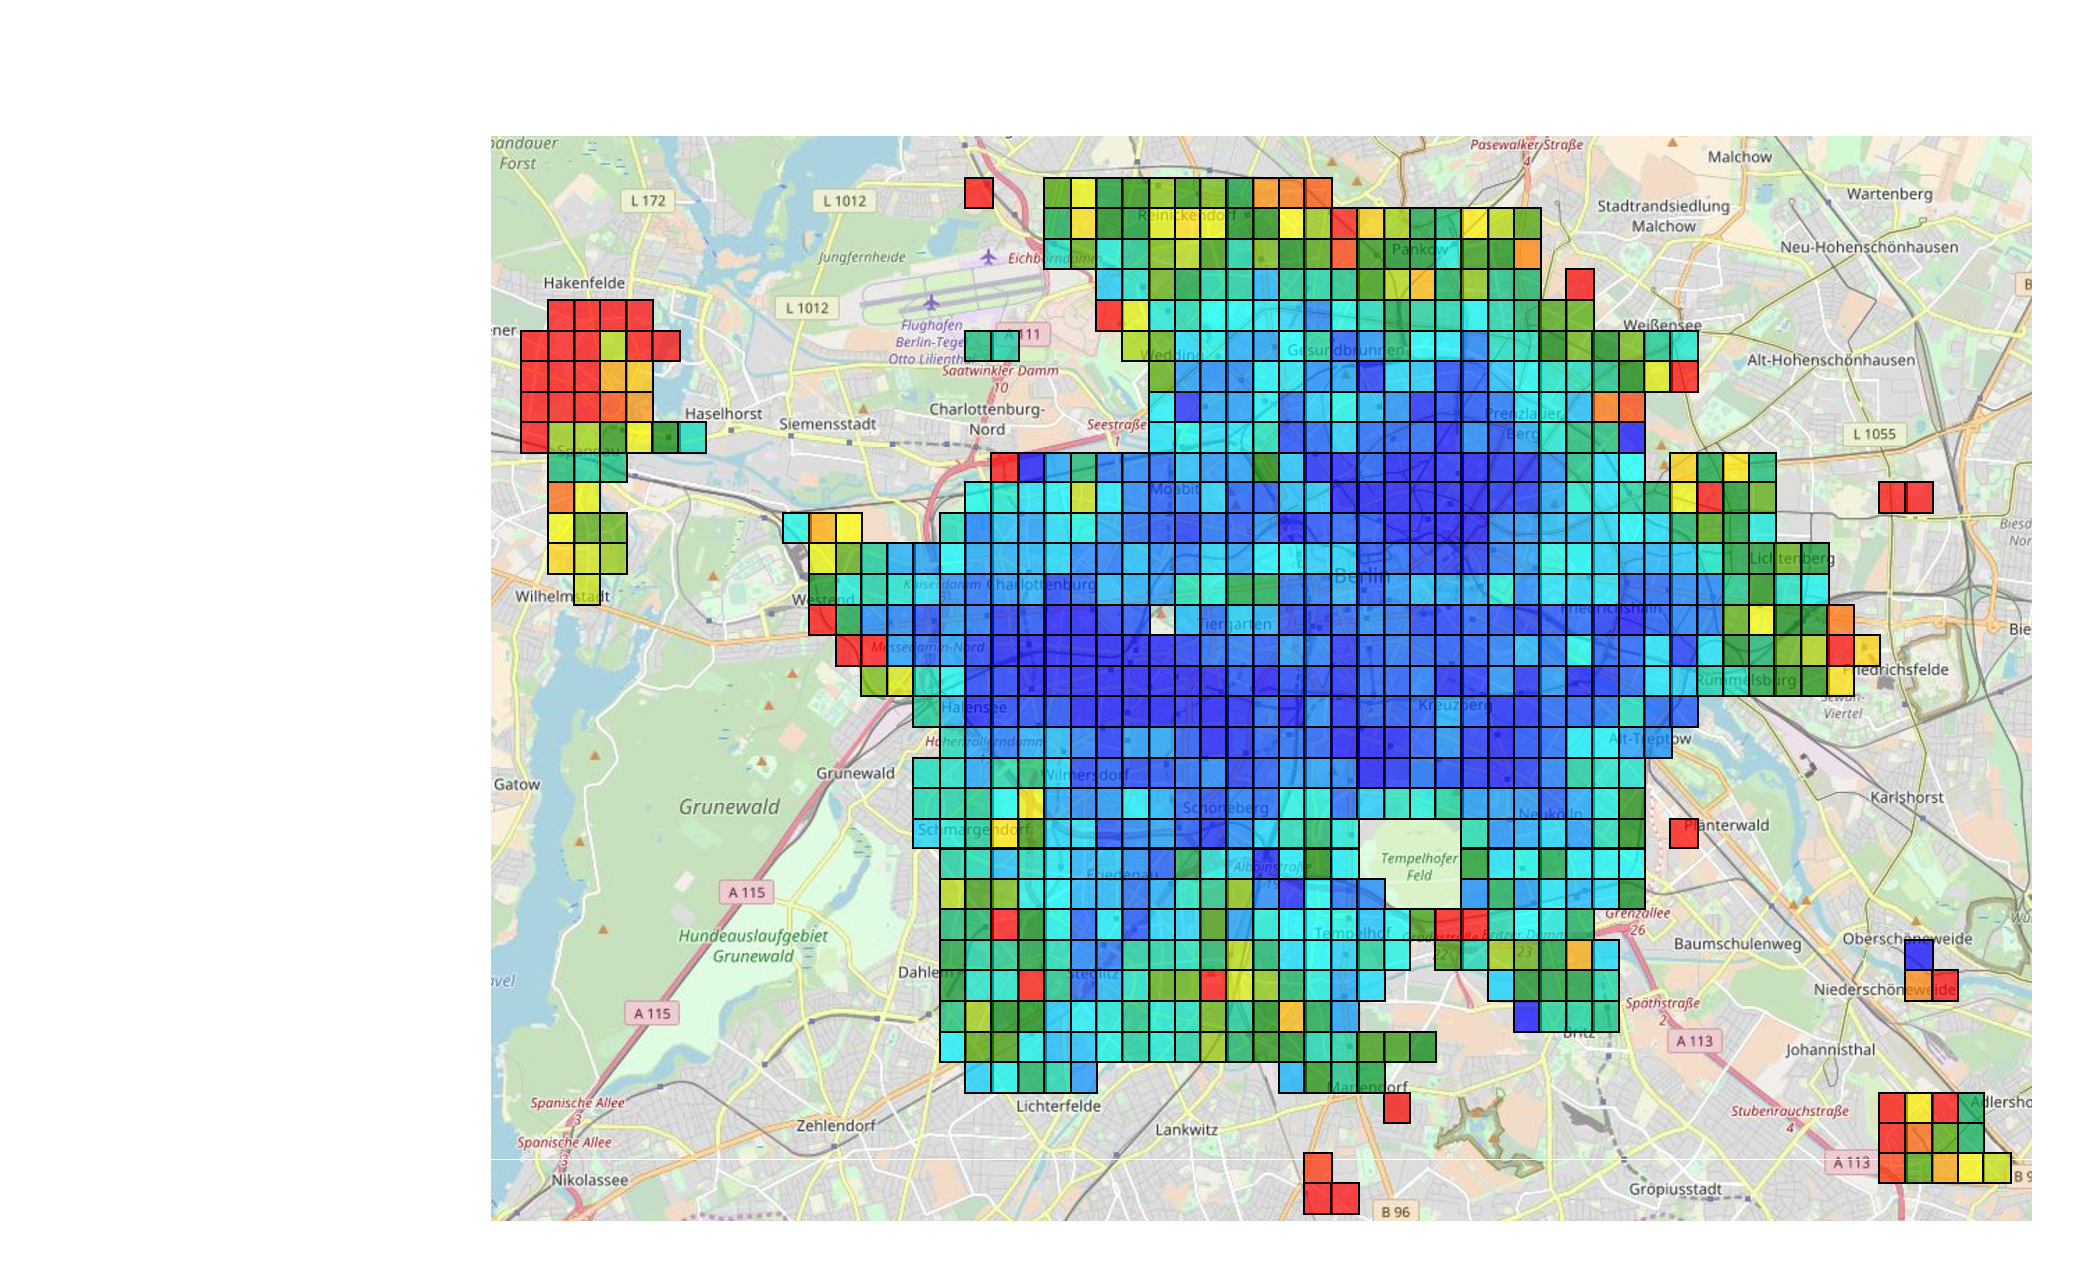
\includegraphics[width=0.495\columnwidth]{figures/BerlinoAvgParking.pdf}
            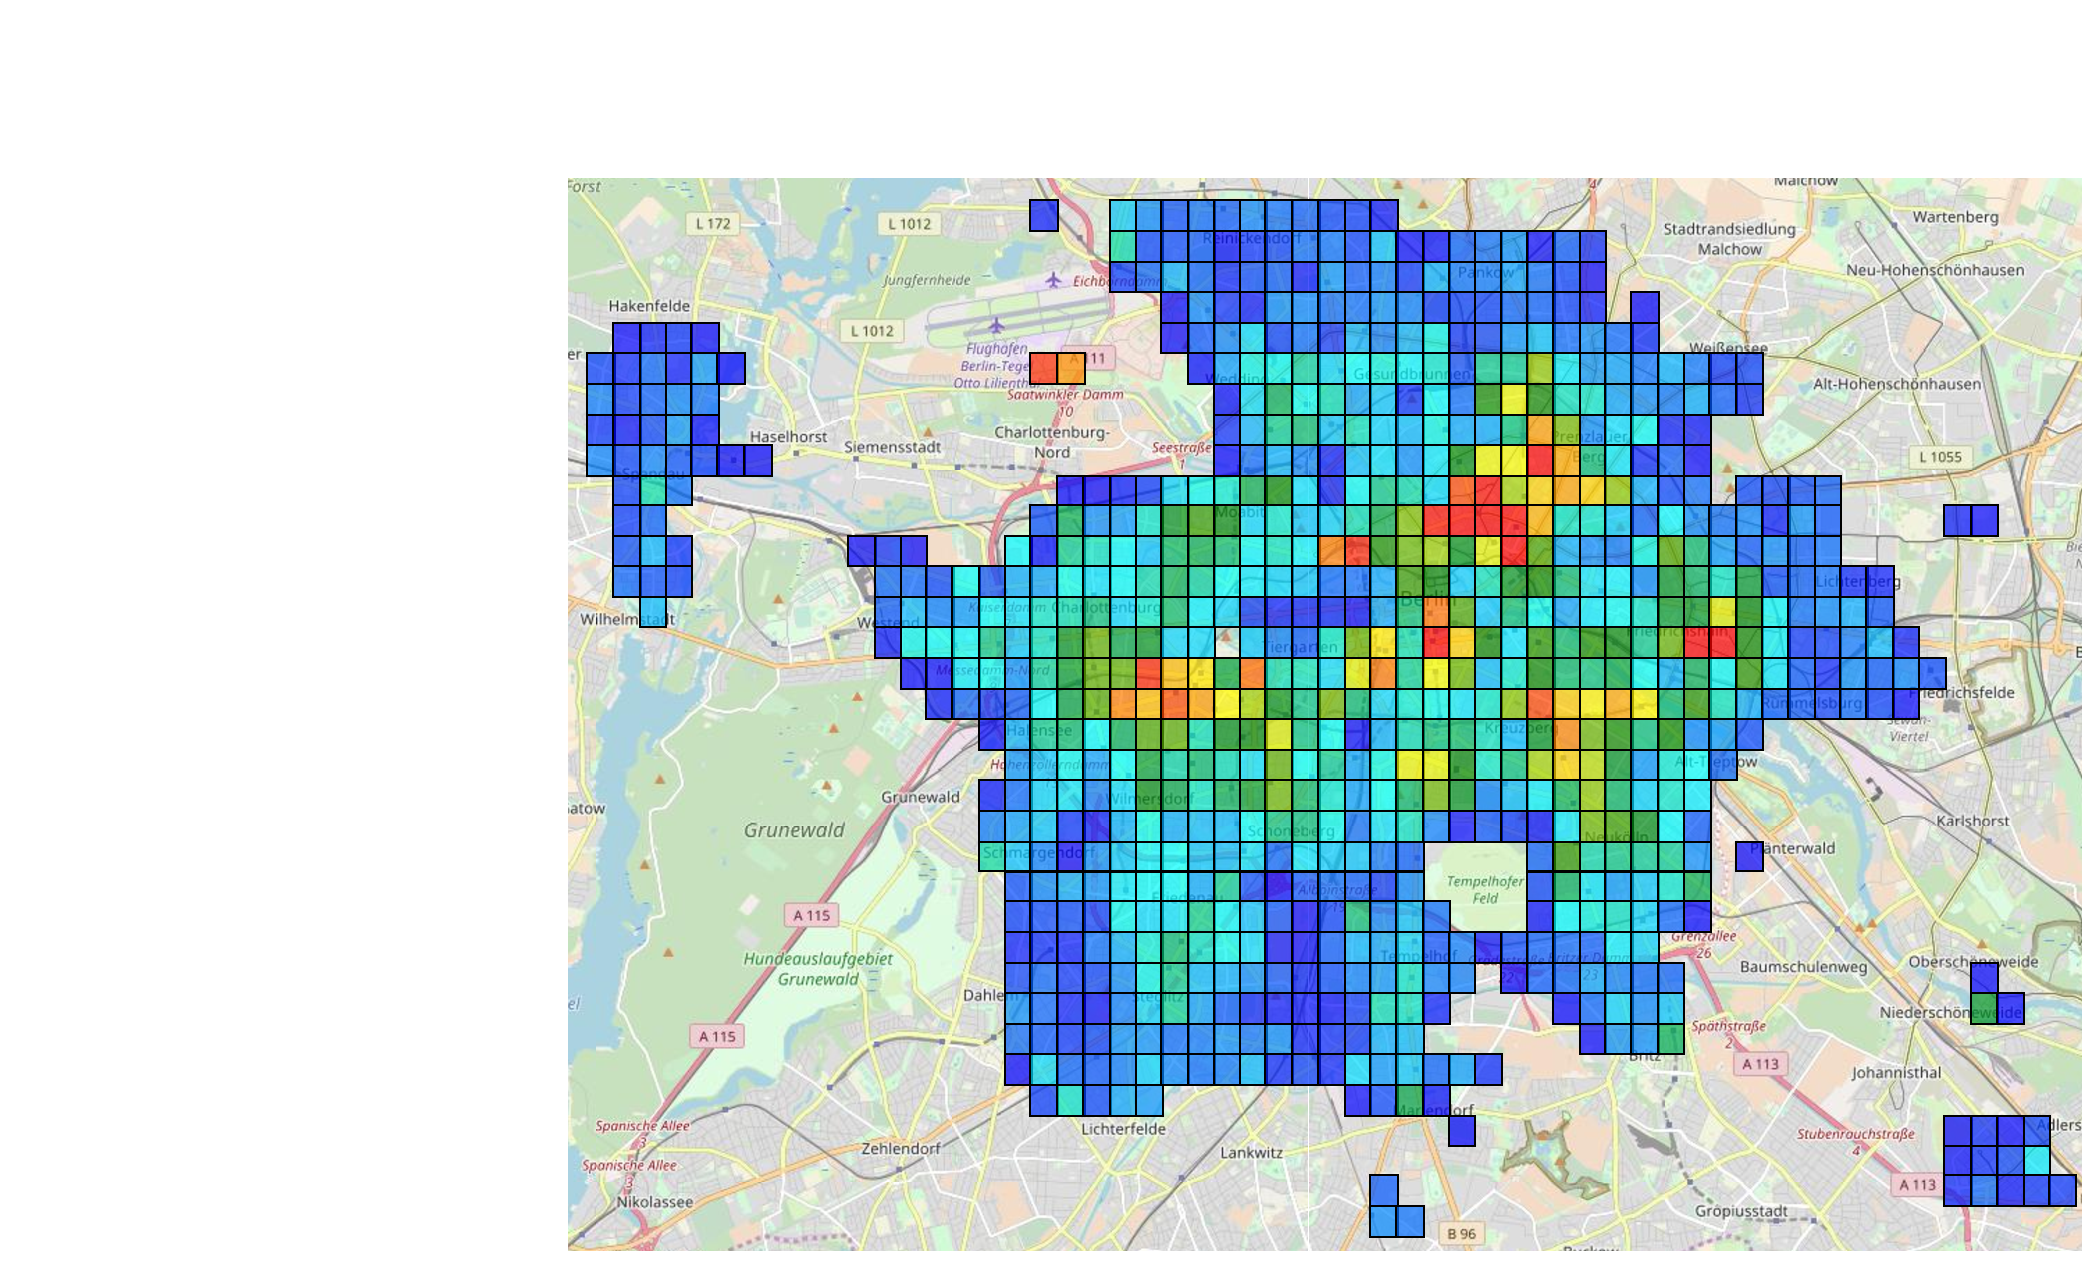
\includegraphics[width=0.495\columnwidth]{figures/BerlinoMaxParking.pdf}                
            \captionsetup{justification=centering}
            \caption{Berlin: average parking time (left) and total number of  parkings (right).}
            \label{fig:heatmap_Berlin}
            \end{center}
        \end{subfigure}
        \begin{subfigure}{\textwidth}
		    \begin{center}
            %\vspace{20pt}
            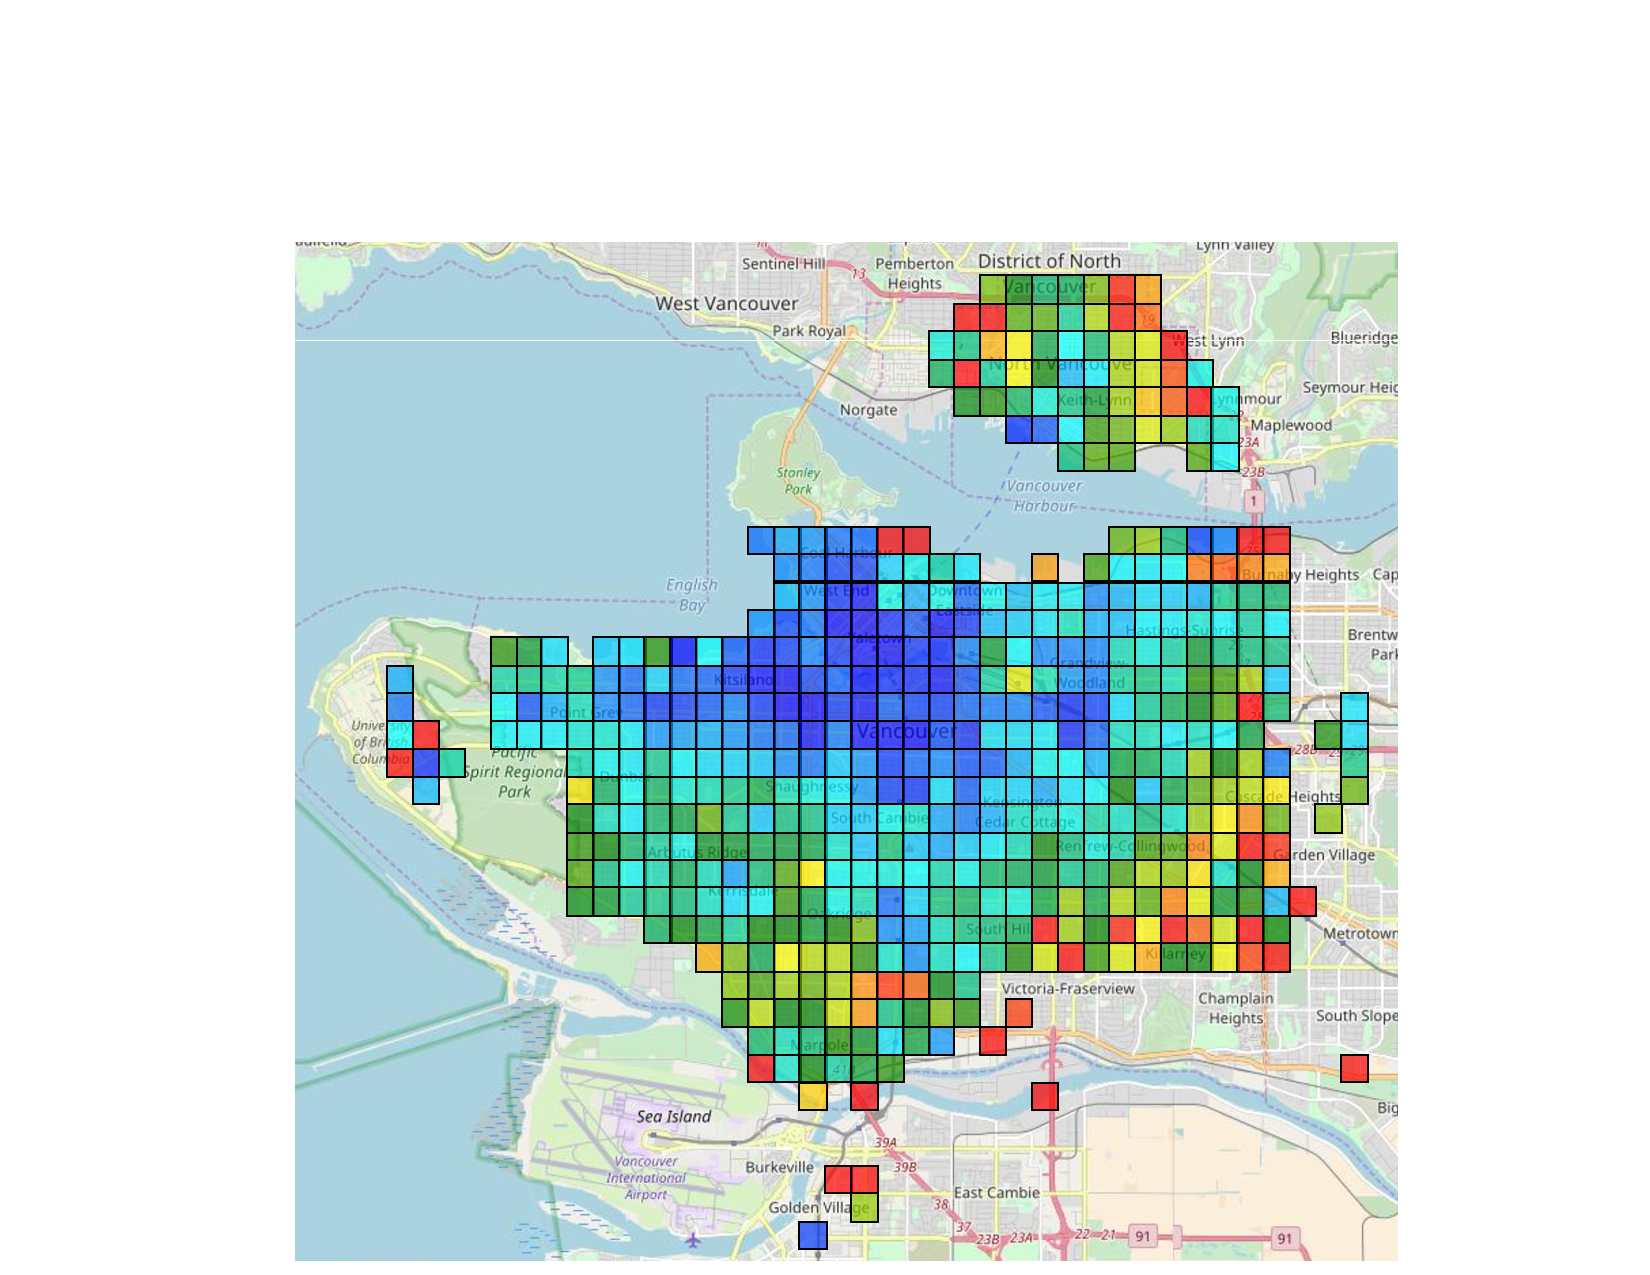
\includegraphics[width=0.495\columnwidth]{figures/VancouverAvgParking.pdf}
            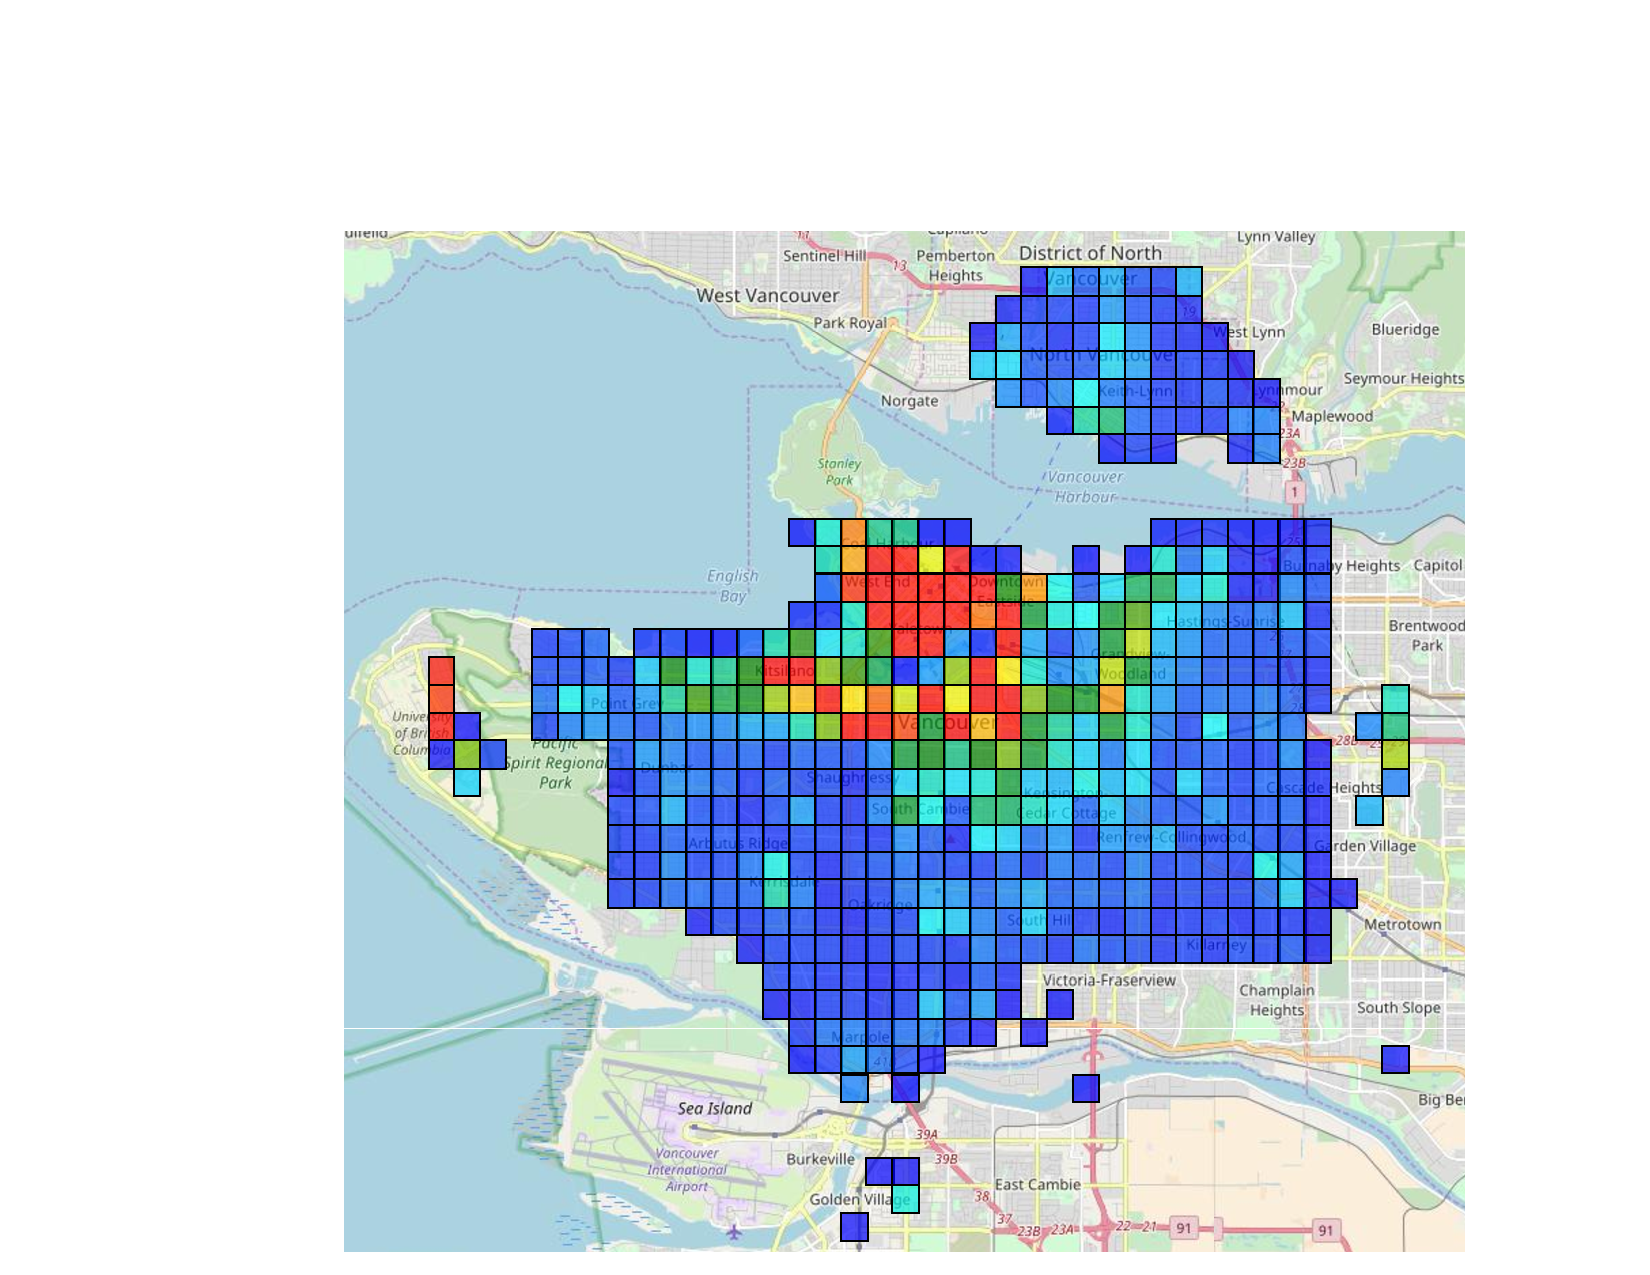
\includegraphics[width=0.495\columnwidth]{figures/VancouverMaxParking.pdf}
            \captionsetup{justification=centering}
            \caption{Vancouver: average parking time (left) and total number of parkings (right).}
            \label{fig:heatmap_vancouver}
            \end{center}
        \end{subfigure}
          \caption{Heat map of average parking time and total number of parking. The warmer the color, the higher the value.}
         \label{fig:heatmaps}
\end{center}
\end{figure*}

To deeply analyze customers' habits, I detail the average number of rentals per hour in figure~\ref{fig:rentals_per_hour}, separately per working-days (WD, solid line) and per weekends (WE, dashed line). Each curve reports the number of rentals for each hour, considering the average number over the same hour in the dataset.
Firstly, notice the usage peaks during commuting times. These happen at different times for different cities, e.g., 8am for Turin, Milan and Berlin vs 7am for Vancouver, following local commuting habits. Secondly, notice how the evening and night usage tend to be larger during  weekends than working days. This reflects the different usage patterns at night, when cars are used to reach areas dense of pubs and nightlife.
At last, observe again the different patterns in different cities. For instance, the average number of rentals in Vancouver and Berlin during weekend mornings is higher than during working days. This does not happen in Italian cities. The charging station placement design must thus weight this different needs and non-stationary patterns.


Given the goals of deriving guidelines for charging station placement policies, I focus now on the characterization of three important metrics:
(i) for how long customers rent a car,
(ii) how far they drive,
(iii) how long cars usually stay parked.
The former two metrics guide the battery discharging properties, while the latter metric is fundamental to understand battery charging opportunities. Given the data-set does not have any information on car position during a rental, I compute the travel distance by assuming the customer went directly from the origin to the destination. This is indeed compatible with the duration of rentals (see below). I use Google Map service to compute a correcting factor to be applied on the euclidean distance, \mc{citare sezione apposita}. 


Figure~\ref{fig:cdf_characterization} reports the Cumulative Distribution Function (CDF) of the rentals duration (top), driving distance (middle) and parking duration (bottom).
The size of the city has a clear impact, with Turin that has the shortest trips, and Berlin the longest. 
Rental duration is in general very short, leading to the intuition that drivers tend to minimize the rental time (and cost). Traveled distance is fundamental to understand the battery consumption: The maximum driving distance sets the minimum battery charge to sustain that trip. Looking at the middle plot in digure~\ref{fig:cdf_characterization}, I observe that in Berlin the longest trips are twice as long as the longest trips in other cities. Therefore, the same battery constraints would not fit for all cities. 

Overall, the limited travelled distance and rental duration suggest people use the car just for the time strictly needed to reach their destinations. Trips are limited by the service area and are thus typically within 15\,km (25\,km for Berlin).

At last, bottom plot of figure~\ref{fig:cdf_characterization} details the duration of the parking periods. Interestingly, 50\% of parkings lasts less than 22 minutes in Berlin, testifying a very high system utilization. In Turin, the median grows to 42 minutes, still showing that most cars are parked for short time. Yet, the long tail of the CDF (note the log scale on x-axis) suggests that there is a sizeable fraction of parkings that last for 5 or more hours. Cars parked in the periphery typically at night, where the demand is lower, belongs to this fraction.
\begin{table}[h!]
\begin{center}
\scriptsize
\caption{Main characteristics of data.\label{tab:summary}}
\setlength\tabcolsep{5pt} % default value: 6pt reduce cell padding
\begin{tabular}{|l|l|l|l|c|c|c|c|c|l|}
\hline
\!\multirow{3}{*}{City} &\!\multirow{3}{*}{Rental}\!& \multirow{2}{*}{Fleet} &  \multicolumn{2}{|c|}{Rental}  &  \multicolumn{2}{|c|}{Rental}  &  \multicolumn{2}{|c|}{Parking}  &\!\multirow{3}{*}{Zones}\!\\ 
 &  & \multirow{2}{*}{Size}  & \multicolumn{2}{|c|}{Time~[min]}  & \multicolumn{2}{|c|}{Dist.~[km]} & \multicolumn{2}{|c|}{Time~[h]} &    \\ \cline{4-9} %&  \multirow{2}{*}{Size[GB]}
 & &  &\!Avg\!&\!Med\!&\!Avg\!&\!Med\!&\!Avg\!&\!Med\!& \\ \hline
\hline
       \!Torino       & 125k & 377 & 21 & 20 & 3.96 & 3.36 & 3:17 & 0:42 & 261 \\ \hline
\!Milano       & 320k & 739 & 25 & 24 & 4.15 & 3.66 & 2:21 & 0:24 & 549 \\ \hline
\!Berlino      & 342k & 900 & 29 & 28 & 6.22 & 5.24 & 2:23 & 0:22 & 833 \\ \hline
\!Vancouver\!  & 317k & 941 & 26 & 24 & 4.70 & 3.98 & 2:54 & 0:22 & 532 \\ \hline

\end{tabular}
\end{center}
\end{table}


\textbf{Takeaway:} car sharing usage is time heterogeneous and non stationary. However, many patterns can be identified. FFCS customers tend to use the system mostly during commuting time and for short trips.

\subsection{Spatial characterization}
\label{sec:dataspace}
The choice of charging station placement has to balance two main factors: place them where cars are (i) frequently parked -- so to maximize the opportunity for charging; and where cars (ii) stay parked for long time -- so to maximize the charging time. Knowing the zones within the city where cars are left parked is fundamental. For this I divide the operative area described in section \ref{sec:5_3_mh_placement}
%For this, we divide the operative area of each city into squared zones, obtained with a grid of 500\,m of side. For each zone, we compute the total number of parkings and the average parking time. 

Figure~\ref{fig:heatmaps} shows the above metrics for Berlin and Vancouver using a heat map -- with blue and red corresponding to the minimum and maximum values, respectively. Focus on Berlin first - figure~\ref{fig:heatmap_Berlin}. Left plot shows the average parking time. Results clearly show that cars stay parked for very short time in busy downtown areas, while cars stay parked for longer time in the periphery (corresponding to the head and tail of the CDF in figure~\ref{fig:cdf_characterization}, respectively).

Conversely, right plot depicts the total number of parkings recorded in each zone. It clearly shows that areas where the majority of rentals/parkings occurs correspond to zones downtown where people frequently drive, drop the car, and then someone else re-rent the same car. 

In a nutshell, in busy areas, the average parking time is short, and number of rentals and parkings recorded is high. This reflects the specific usage of FFCS according to which cars move to downtown areas in the morning, then are rented to move within central areas, and finally are driven back to the periphery at the end of the day.
Similar results apply to all cities -- see Fig.~\ref{fig:heatmap_vancouver} which details Vancouver statistics.

In the following I leverage this knowledge obtained by actual data, to compare the design of and optimize different charging station placement policies.


\textbf{Takeaway:} Periphery zones are characterized by a long parking time, while central areas are characterized by many parkings which last a short time.


